% JF -> XM : this chapter lacks structure

\chapter{Designing the generation chain}
\label{cpt:frame}

An important part of the specification of the ARMv6 instruction set
(the behavior of 147 instructions and 24 addressing modes)
is defined in the ARMv6 reference manual using a pseudo-code notation.
As explained in the previous chapters,
the Coq formal model of ARM instructions and their C representation for \simlight
are systematically derived from this pseudo-code.
Most instructions are described using more than 10 lines of pseudo-code. 
Manually translating them one by one would be a repetitive and error-prone task. 
% JF->XM: A bit redundant: pseudo-code is, by definition, semi-formal.
% Since the pseudo-code of instructions is in semi-formal style,
We then built a automatic generator, which takes the pseudo-code
of instructions as input and returns their representations in Coq and in C.
The corresponding generation chain is presented in this chapter.

% In the previous two chapters we introduce the representation of an instruction
% operation in Coq language and in C language separately.

% Previously, we present how to translate manually a instruction
% operation pseudo-code into Coq formal representation and C interpretation.
% We realized it is possible to obtain the two kinds of representation of every
% instruction in an automatic and systematic way.
% The following sections introduce how to build such automatic code generator
% for ARMv6 instruction set.

\selectlanguage{french}
\section*{Résumé}

\begin{resume}
Une partie importante de la spécification du jeu d'instructions de l'ARMv6
(le comportement des 147 instructions et des 24 modes d'adressage)
est définie dans le manuel de référence de l'ARMv6 au moyen d'une notation
en pseudo-code.
Ainsi qu'on l'a expliqué dans les chapitres précédents,
le modèle formel Coq des instructions ARM et leur représentation en C 
pour \simlight sont systématiquement dérivés à partir de ce pseudo-code.
Pour la plupart des instructions, la description en pseudo-code fait plus de 10 lignes.
Leur traduction à la main serait une tâche répétitive et sujette à erreurs.
Nous avons donc construit un générateur automatique,
prenant en entrée le pseudo-code des instructions et retournant leur
réprésentation en Coq et en C,
et la chaîne de génération correspondante fait l'objet de ce chapitre. 
\end{resume}

\selectlanguage{english}

%\section{Requirement from SimSoC}
%\subsection{The new version of ARM architecture}

% For the C programmers, things are simple: all ARM architectures offer a regular, 32-bit with flat addressing programming model. As long as you stay with C source code, the only difference you may see is about endianness and performance. Most ARM processors (even old models) can be both big-endian and little-endian; the choice is then made by the logic board and the operating system. Good C code is endian neutral: it compiles and works correctly, regardless of the platform endianness (endian neutrality is good for reliability and maintainability, but also for performance: non-neutral code is code which accesses the same data through pointers of distinct sizes, and this wreaks havoc with the strict aliasing rules that the compiler uses to optimize code).

% The situation is quite different if you consider binary compatibility (i.e. reusing code which has been compiled once):

%     There are several instruction sets:
%         the original ARM instruction set with a 26-bit program counter (very old, very unlikely to be encountered nowadays)
%         the ARM instruction set with a 32-bit program counter (often called "ARM code")
%         the Thumb instruction set (16-bit simplified opcodes)
%         the Thumb-2 instruction set (Thumb with extensions)

% A given processor may implement several instruction sets. The newest processor which knows only ARM code is the StrongARM, an ARMv4 representative which is already quite old (15 years). The ARM7TDMI (ARMv4T architecture) knows both ARM and Thumb, as do almost all subsequent ARM systems except the Cortex-M. ARM and Thumb code can be mixed together within the same application, as long as the proper glue is inserted where conventions change; this is called thumb interworking and can be handled automatically by the C compiler.

% The Cortex-M0 knows only Thumb instructions. It knows a few extensions, because in "normal" ARM processors, the operating system must use ARM code (for handling interrupts); thus, the Cortex-M0 knows a few Thumb-for-OS things. This does not matter for application code.

% The other Cortex-M know only Thumb-2. Thumb-2 is mostly backward compatible with Thumb, at least at assembly level.

%     Some architectures add extra instructions.

% Thus, if some code is compiled with a compiler switch telling that this is for an ARMv6, then the compiler may use one of the few instructions with the ARMv6 has but not the ARMv5. This is a common situation, encountered on almost all platforms: e.g., if you compile C code on a PC, with GCC, using the -march=core2 flag, then the resulting binary may fail to run on an older Pentium processor.

%     There are several call conventions.

% The call convention is the set of rules which specify how functions exchange parameters and return values. The processor knows only of its registers, and has no notion of a stack. The call convention tells in which registers parameters go, and how they are encoded (e.g. if there is a char parameter, it goes in the low 8 bits of a register, but is the caller supposed to clear/sign-extend the upper 24 bits, or not ?). It describes the stack structure and alignment. It normalizes alignment conditions and padding for structure fields.

% There are two main conventions for ARM, called ATPCS (old) and AAPCS (new). They are quite different on the subject of floating point values. For integer parameters, they are mostly identical (but AAPCS requires a stricter stack alignment). Of course, conventions vary depending on the instruction set, and the presence of Thumb interworking.

% In some cases, it is possible to have some binary code which conforms to both ATPCS and AAPCS, but that is not reliable and there is no warning on mismatch. So the bottom-line is: you cannot have true binary compatibility between systems which use distinct call conventions.

%     There are optional coprocessors.

% The ARM architecture can be extended with optional elements, which add their own instructions to the core instruction set. The FPU is such an optional coprocessor (and it is very rarely encountered in practice). Another coprocessor is NEON, a SIMD instruction set found on some of the newer ARM processors.

% Code which uses a coprocessor will not run on a processor which does not feature that coprocessor, unless the operating system traps the corresponding opcodes and emulates the coprocessor in software (this is more or less what happens with floating-point arguments when using the ATPCS call convention, and it is slow).

% To sum up, if you have C code, then recompile it. Do not try to reuse code compiled for another architecture or system.

% \subsection{A more convenient way to obtain code}
% JF -> XM: moved to the beginning of the chapter

\section{Architecture}
\label{sec:overall}
%copy from cpp11


\begin{figure}
\hfil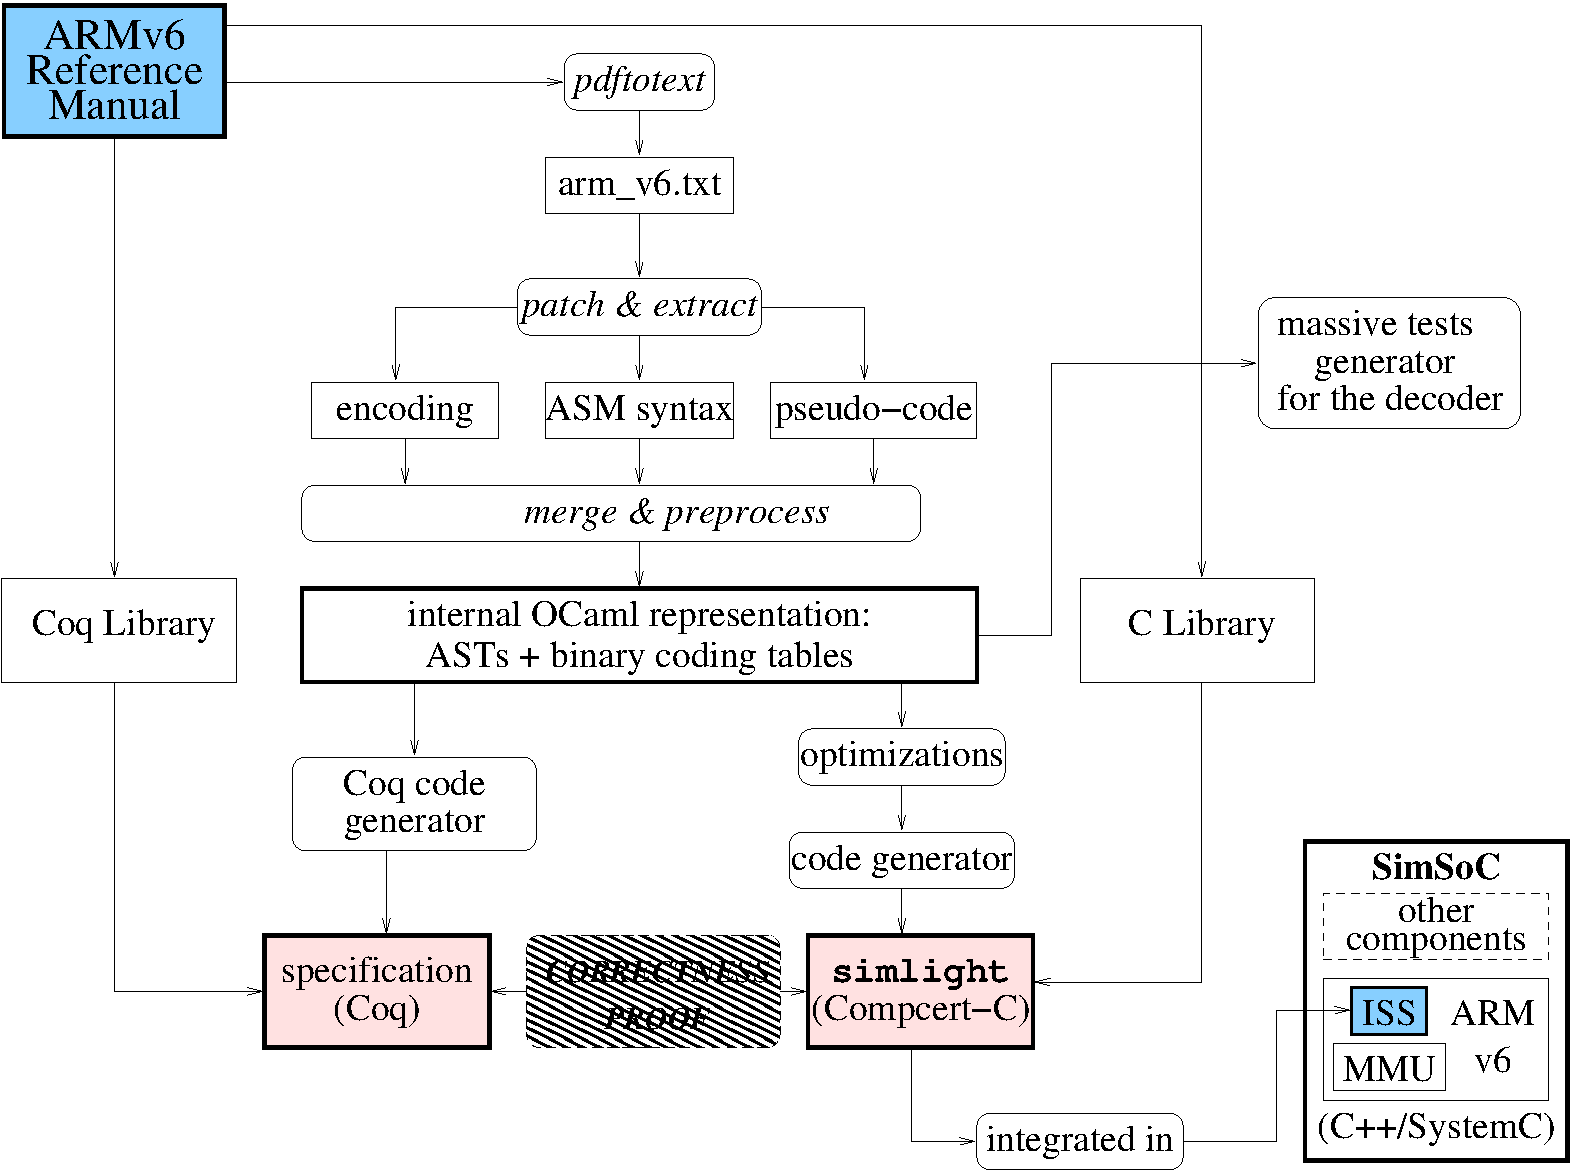
\includegraphics[width=\linewidth]{fig/fullarchi.pdf}
\caption{Overall generation chain}
\label{fig:arch}
\end{figure}

The overall architecture of the automatic generator is given in figure
\ref{fig:arch}.
% % JF -> XM: the text commented out here is redundant at this point.
% The requirement of \simsoc, the simulator, is to take the new architecture ARMv6
% into account, to prove such ARMv6 simulator is correct and the C simulator
% behavior fully corresponding to the document,
% and then integrate the proved correct simulator into \simsoc.
% Our idea is to first have a formal model of ARMv6 simulator including the ISS,
% a main processor, a simple memory model, a decoder, and a simulation loop.
% Then we compare the formal model with the C specifications of the simulator.
% This idea will be detailed in Section \ref{sec:gi}.
% Then the first task to do is to formalize the ARMv6 model in Coq
% ~\cite{coqmanual}. 
% Both formal specification in Coq and C description are relied on ARMv6 Reference
% Manual which
% contains 28500 lines.
% To have so many contents formalized by hand will be a tedious and error-prone
% work.
% We notice that the reference is basically written in natural language,
% but some parts are in pseudo-formal descriptions. 
% Then it is possible for us to automatically parse and manipulate them.
% The following introduces this automatic code generation.

The figure shows there are three data flows coming from manual.
Two are going to be formalized manually; the other one part
is going be interpreted and merged automatically.
%
% % JF->XM: no need for the next sentence..
% The reference is manually written.
%
% % JF->XM: dangerous to say the following this way: all our work could be compromized...
% which is not completely correct in any sense.
% We have found several bugs in the document by reading and by testing the 
% generated simulator.

More specifically, we can see the data flow from ARMv6 Reference Manual 
to the Coq model and to the simulation code. 
Some patches are needed from the textual version of the
reference manual because the latter contains some minor bugs
(see below).

Three kinds of
information are extracted for each ARM operation: its binary encoding format,
the corresponding assembly syntax, and its body, which is an algorithm operating
on various data structures representing the state of an ARM: registers, memory,
etc., according to the fields of the operation considered. This algorithm may 
call general purpose functions defined elsewhere in the manual, for which we provide
a \compcert C library to be used by the simulator and a Coq library defining
their semantics. The latter relies on Integers.v and Coqlib.v from the \compcert
library which allows us, for instance, to manipulate 32-bits representations of
words. The result is a set of abstract syntax trees (ASTs) and binary coding
tables. These ASTs follow the structure of the (not formally defined) 
pseudo-code. 

In the end, three files are generated: a Coq file specifying the behavior of all
operations (using the aforementioned Coq library), a \compcert C file to be
linked with other components of \simsoc (each instruction can also be executed
in stand-alone mode, for test purposes for instance)
and a Coq files representing each instructions in \compcert C AST
to be used for correctness proof.

% % JF-> XM: irrelevant subsection title
% \subsection{A reusable development framework}

% % JF->XM: redundant
% The back-end automatic code generator is shown in Figure~\ref{fig:arch}.
%input

\section{Analysis of the ARM reference manual}

The whole process starts with the ARMv6 reference manual {\stt ARM DDI 0100I}
\cite{arm6refman}. 
% % JF->XM, about next sentence: 
% % in a thesis, we are interested in the conclusions, what you get at then end,
% % and not in the process of getting it (unless it is a thesis on psychology
% We go through the manual roughly. 
The relevant chapters for us are:
\begin{itemize}
\item
\texttt{Programmer's Model} introduces the main features in ARMv6 architecture,
the data types, registers, exceptions, etc;
\item
\texttt{The ARM Instruction Set} 
explains the instruction encoding in general and puts the instructions in
categories;
\item
\texttt{ARM Instructions} lists all the ARM instructions in ARMv6 architecture
in alphabetical order and \texttt{ARM Addressing modes} gives all the five kinds 
of addressing modes;
\item
\texttt{Glossary} gives all the definitions of key words in ARMv6. We use it
as a reference to define manually the common functions.
\end{itemize}

% % JF->XM, about next sentence: 
% % in a thesis, we are interested in the conclusions, what you get at then end,
% % and not in the process of getting it (unless it is a thesis on psychology
% Then let us look carefully into Chapter \texttt{ARM Instructions} 
% in the reference manual. 

There are 147 ARM instructions in the ARMv6 architecture. 
For each instruction, the manual gives its encoding
table, its syntax, a piece of pseudo-code explaining its own
operation, its exceptions, usage, and notes.  Except the semi-formal
pseudo-code, everything else is written in nature language. 

% % JF->XM: not useful in this chapter
% An example of pseudo-code of instruction ADC is in figure~\ref{fig:adcpc}.

%preparing
% % JF->XM, about next sentence: 
% % in a thesis, we are interested in the conclusions, what you get at then end,
% % and not in the process of getting it (unless it is a thesis on psychology
% Using Linux command {\stt pdftotext} we are able to obtain a 28,500 lines 
% text file from the original pdf reference manual.

The first step is extraction and patching. 
We extract three files from the reference manual: 
a 2100 lines file containing the pseudo-code, a 800 lines file
containing the binary encoding tables, and a 500 lines file containing the
ASM syntax. 
Other than these three extracted files, there are still useful information left
in the document which cannot be automatically extracted.
% % JF->XM, about next sentence: 
% % in a thesis, we are interested in the conclusions, what you get at then end,
% % and not in the process of getting it (unless it is a thesis on psychology
% These informally described part will be later written by hand.
%
This is the case for
the arithmetic functions given in chapter \texttt{Glossary},
and for
the validity constraints information required by the decoder generator.
The corresponding information is manually translated into
a 300 lines OCaml file.

Before extraction, a patch is necessary for the main text file. This
patch is obtained from reading the manual or feedback from the generation result.
The patch fixes the mistakes in the original document, such as misspelling
function names, unclosed parenthesis, missing line, etc.
Most of these bugs were found by running the generator or
testing the generated simulator.
The differences are kept in a diff file,
so that they could be submitted to the ARM company and confirmed.

%preprocessing
Then each extracted file is parsed with the corresponding parser.
The one to parse pseudo-code is more complicated. Two preliminary phases solve
issues related to line breaks and indentation, given that indentation defines
the blocks in Python-like way. 

Then, a classical lexer parser combination builds the abstract syntax trees (ASTs). 
We have built our own ASTs for intermediate representation which contains the
elements representing both instructions and their addressing mode.

\section{Intermediate representation}

% \jf{Give here the main datatypes of the 
% ``internal OCaml representation, AST + binary code'' mentioned in 
% Figure~\ref{fig:arch}
% with a few comments on these}

The abstract syntax of the intermediate representation expressions
is given in Figure~\ref{fig:irexp}.
The corresponding OCaml definition is an inductive data type.
The type of expression supports numbers in different bases,
conditional expressions, function calls, binary operations, 
ranges (e.g. Rn[31:0] indicate the range of bits 0 to 31 of register Rn),
and the particular expression of ARM registers 
(e.g. \texttt{CPSR}, \texttt{SPSR}, and \texttt{Reg}), memory and coprocessor.
Additionally, two key words are included:
\texttt{Unaffected} which indicates the item is
not changed by an operation,
and \texttt{Unpredictable\_exp} which represents an unreliable instructions result.
The evaluation of expression \texttt{Unpredicatable\_exp} and \texttt{Coproc\_exp}
can bring side-effect. 

\begin{figure}
\begin{alltt}
  \textit{exp} ::= num
        | bin
        | hex
        | float
        | if \textit{exp} then \textit{exp} else \textit{exp} 
        | fun (\textit{exp list})
        | \textit{exp} binop \textit{exp}
        | \textbf{CPSR}
        | \textbf{SPSR} \textit{mode option}
        | \textbf{Reg} \textit{mode option}
        | var
        | \textit{exp} of \textit{range}
        | \textbf{Unaffected}
        | \textbf{Unpredictable\_exp}
        | \textbf{Memory} \textit{size}
        | \textbf{Coproc\_exp} \textit{exp list}
  \textit{mode} ::= Fiq | Irq | Svc | Abt | Und | Usr | Sys
  \textit{range} ::= bit | flag | index
  \textit{size} ::= byte | half | word
\end{alltt}
\caption{The abstract syntax of intermediate representation expressions}
\label{fig:irexp}
\end{figure}

Figure~\ref{fig:irstm} defines the abstract syntax of instruction statements,
which is defined in type \textit{inst}.
The C-style structural statements are supported: blocks, assignments,
conditional statements, loops (while loop and for loop), assert, case, and return.
Special function calls related to processor and coprocessor are presented
individually.
Within statements, \texttt{Unpredictable} appears again.
In pseudo-code, \armrf{UNPREDICTABLE} is used as the expression of right value
in the assignment (e.g. \armrf{data = UNPREDICTABLE}), or as the statement of call to
the function (e.g. \armrf{if...then...else UNPREDICTABLE}).


\begin{figure}
\begin{alltt}
  \textit{inst} ::= block \textit{inst list}
         | let \textit{fun} (\textit{args}) = \textit{inst list}
         | \textbf{Unpredictable}
         | \textit{exp} = \textit{exp}
         | if (\textit{exp}) \textit{inst} \textit{inst option}
         | Proc_function \textit{exp list}
         | while (\textit{exp}) \textit{inst}
         | assert \textit{exp}
         | for (string) \textit{inst}
         | Coproc_function \textit{exp list}
         | case (\textit{exp}) \textit{inst list}
         | return \textit{exp}
\end{alltt}
\caption{The abstract syntax of intermediate representation statements}
\label{fig:irstm}
\end{figure}

\section{Code generation}
\label{sec:codegen}

On the formal specification side (left side of the generation chain in Figure~\ref{fig:arch}),
we directly use the ASTs for generating Coq code. 

% % JF->XM: I guess that this flattening makes another interesting difference
% % between \simlight and the Coq model.
% % E.g. for ADC, there are adressing modes?
% % Which one is taken?
% % Was it easy to deal with?
% % Or is is for \simlight 2 only???

% % XM -> JF : flattening is for \simlight 2 only.

For the generation of C source code, we can make an easy optimization to generated the 
second version of \simlight,
in order to improve the simulation speed:
as we mentioned in Section~\ref{sec:slv62},
\textit{flattening} is one way of improving the simulation performance.
We {\em flatten} some instructions with their addressing mode
%\margjf{1}{XM, see important comment in latex source}. 
When an instruction $A$ can be used in an addressing mode $B$,
the generation provides a combined instruction $AB$.
This simple optimization can make the generation steps shorter and the generated
code faster. And after flattening, the notions of addressing modes disappear.

This flattening step is achieved by four operations:
\begin{itemize}
\item
  Inlining the addressing mode to instruction operation code;
\item
  Appending the validity constraint information;
\item 
  Merging the encoding table of the instruction and addressing mode case
  (example in figure \ref{fig:flatten})
\item
  Merging the ASM syntax of the instruction and addressing mode case
\end{itemize}

%\hide{
%\newcommand{\jfdots}{$\ldots$}
\newcommand{\jfdots}{$.\,.\,.\,$}
\begin{figure*}\centering
\small
\begin{tabular}{|c|c|c|c|c|c|c|c|c|c|}
\multicolumn{10}{c}{\small\em (a) binary encoding of the {\stt ADC} instruction}\\
\hline
31 \jfdots 28 & 27 26 & 25 & 24 \dotfill 21 & 20 & 19 \jfdots 16 & 15 \jfdots 12 & \multicolumn{3}{c|}{11 \dotfill 0} \\\hline
\stt cond & \stt 0~0 & \stt I & \stt 0~1~0~1 & \stt S & \stt Rn & \stt Rd & \multicolumn{3}{c|}{\stt shifter\_operand} \\
\hline
% \multicolumn{10}{c}{~}\\
\multicolumn{10}{c}{\small\em \phantom{\LARGE I}(b) binary encoding of the ``logical shift left by immediate'' operand\phantom{\LARGE I}}\\
\hline
31 \jfdots 28 & 27 26 & 25 & 24 \dotfill 21 & 20 & 19 \jfdots 16 & 15 \jfdots 12 & 11 \dotfill 7 & 6 \jfdots 4 & 3 \jfdots 0 \\\hline
\stt cond & \stt 0~0 & \stt 0 & \stt opcode & \stt S & \stt Rn & \stt Rd & \stt shift\_imm & \stt 0~0~0 & \stt Rm \\
\hline
% \multicolumn{10}{c}{~}\\
\multicolumn{10}{c}{\small\em \phantom{\LARGE I}(a+b) resulting binary encoding of the flattened instruction\phantom{\LARGE I}}\\
\hline
31 \jfdots 28 & 27 26 & 25 & 24 \dotfill 21 & 20 & 19 \jfdots 16 & 15 \jfdots 12 & 11 \dotfill 7 & 6 \jfdots 4 & 3 \jfdots 0 \\\hline
\stt cond & \stt 0~0 & \stt 0 & \stt 0~1~0~1 & \stt S & \stt Rn & \stt Rd & \stt shift\_imm & \stt 0~0~0 & \stt Rm \\
\hline
\end{tabular}

\caption{Flattening the ADC instruction with the shift left by immediate operand}
\label{fig:flatten}
\end{figure*}
%}

There are some specific points for the pre-processing phase:
\begin{itemize}
\item
  We can have a \emph{base register write-back} specification, saying that
  the base register which is used in address calculation will be modified.
  We have this case when \armrf{Rd == Rn}.
  The result is \armrf{UNPREDICTABLE} if the base register is PC.
  The base register write-back is disabled in M2, M3, M4 addressing modes.
  %and replaces the expression of write-back to the end of the
  %operation due to the rule of write-back.
\item 
  Some functions are reshaped depending on the number of arguments
  and the operation performed on them.
  For example, \armrf{CarryFrom(a + b)} is replaced by \texttt{CarryFrom\_add2(a, b)},
  which indicates that the carry is calculated from the ``add'' of two arguments.
\item
  Some \textit{if} or nested \textit{if} expressions concern occur when there is
  at least one \armrf{UNPREDICTABLE} in the branches.
  They are merged by pre-processing in order to remove repetitive branches,
  so that we get
  at most one \armrf{UNPREDICTABLE} in a then-branch.
  
\end{itemize}

%code generating
% % JF-XM: not much information there, propose to remove it
% From the cleared up intermediate representation to the object code, the code
% generator is basically a mapping. 
% Actually, we use a generator only for parts that are related to the
% instruction list (255 entities described in a same way). Indeed, it is not worth
% using a generator for something that is not repetitive because the generator
% would be longer than the generated code.

\section{Formats for C code}

% \jf{Explain here what we discussed: 
% generate C code in textual or \compcert AST format.
% Pros and cons. 
% Parser and pretty-printer.
% May add a figure if time available?}

To detail the generation of C implementations,
we present a new Figure~\ref{fig:genc}.
In the first line, 
the C source code is generated directly from the optimized intermediate
representation, and then go through the C parser provided by \compcert 
and a C to
\compcert C interpretation. 
Both instructions and library are parsed into \compcert C ASTs.
This result is integrated into the ARM simulator in SimSoC.
The second line translates the intermediate representation AST
into \compcert C AST, and then pretty print into Coq representation and C code too.
From the AST translation, only the instructions are obtained.
The result in Coq representation is used in the correctness proofs.
By comparison,
the pretty printed C code and the \compcert code obtained from the C parser are
identical to each other. Parsing to \compcert C does not lose
any information, which means the subset of C, \compcert C, is large enough to
be fulfill the requirement of ARM instructions.

\begin{figure}
\hfil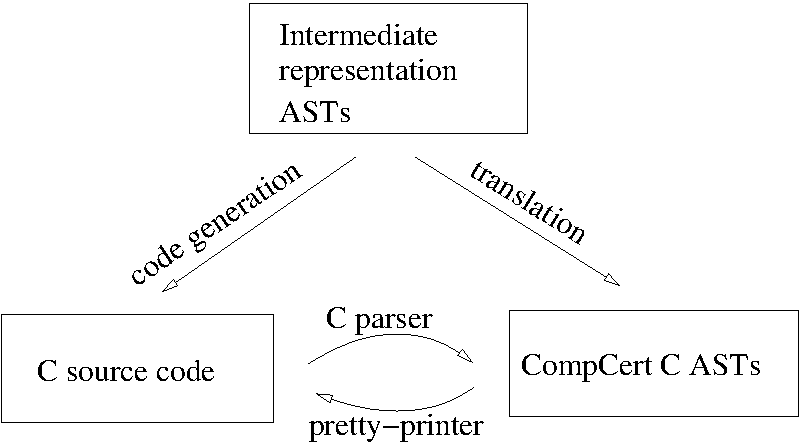
\includegraphics[width=0.7\linewidth]{fig/genc.pdf}
\caption{Generating C code}
\label{fig:genc}
\end{figure}

% \jf{Oh, starting on next Chapter, just saw the following in blue color, which
% I then moved from there to here -- it is a much better place.
% Note that the English (and the contents) of this blue text needs improvement.
% It contains part of what we discussed.
% Try to change/update it, using what follows.
% }

Proofs are to be performed on \compcert C ASTs, 
so the more direct way such ASTs are obtained, the better,
is in order to avoid possible mistaken auxiliary tranformations 
as far as we can
(no proofs have been performed on parsers and pretty-printers
for \compcert C).
But it makes sense only for automatically generated C programs:
writing ASTs by hand would be much too heavy and tedious.
Therefore, we have two cases to consider.
C libraries are written in textual format and parsed 
by the \compcert C front-end,
while C instructions automatically derived from the pseudo-code
are basically \compcert C ASTs
and pretty-printed for a manual double-check in a readable form.
As a result, for proofs,
the \compcert C parser is in the trusted code base (TCB) for libraries,
not for automatically derived code.
If we execute the corresponding programs using the \compcert C compiler,
the TCB is the same.
If we execute the corresponding programs using another compiler,
the TCB includes the pretty-printer and this compiler as well.

As a final remark on the reliability of the \compcert C parser
and the pretty-printer,
we also checked that, for all the generated code,
parsing then pretty-printing yields the original code.

\section{Mistakes in the ARM reference manual }

%% JF -> Vania : TODO : ENGLISH TO BE POLISHED IN THIS SECTION

While building the generators described in this chapter,
we discovered
several bugs in reference manual.

\begin{itemize}
\item
  Important lines were missing in instructions pseudo-code. In the
  operation of many conditional instructions, the condition checking
  was ignored. This leads to a fatal error when the execution
  condition is not satisfied.
  Also for some of load/store instruction, reading the base
  \texttt{address} is missing, which should be the content of register
  \texttt{Rn}. Without initialization, it is impossible to give
  \texttt{address} a value to start with.
\item
  The case sensitivity gave the same spelling different meanings.  
  For example, in the formal model, the binary operation $and$ applies to type
  Boolean, but operation $\mathit{AND}$ in capital is of type $word
  \rightarrow word \rightarrow word$.  Mixing two of them will lead to
  a type mismatch.
\item
  Information was lacking in keywords. For example, in general,
  \texttt{SignExtend} propagates the sign bit of its argument to 32
  bits, but for instruction \texttt{BLX(1)}, \texttt{SignExtend}
  is for the 24-bit signed to 30 bits.
\item
  Mismatched parenthesis.
%% XM : TODO. Retrieve what I meant.
% \item
%   Using deanery notation for binary system.
\item
  Wrong order of expressions in some operations. 
\item 
  In assembly syntax, the expression of register content \texttt{Rx}
  had to be replaced by \texttt{<Rx>}.
\end{itemize}


These bugs have been reported to ARM group.
The feedback was that all these bugs are fixed in ARMv7 reference
manual. 
% Then the effort to change our framework for ARMv7 architecture would
% be not much. And by reading the new reference manual, the description
% of instruction set is much more formal and better structured.
% Thus, the pre-process and other remedial transformation steps can be
% avoided.x


% JF BEGIN MOVED FROM CHAP 2

% {\color{blue}
% \noindent
% \texttt{BEGIN to be moved and updated somewhere}

% % XM
% % When we want to obtain the \compcert C representation of ARMv6 model, 
% % there are two ways. First, use the \compcert C provided converter to generate \compcert
% % C code from \simlight C file, which is not a verified translation step in \compcert.
% % JF -> XM : warning, what you wrote was misunderstood
% % JF 
% The \compcert C representation of ARMv6 can be presented in two ways:
% in textual form or using an AST (Abstract Syntax Tree).

% Two options can then be considered.
% The first is to use the converter provided by \compcert C to generate \compcert 
% C code from \simlight C file, which is not a verified translation step in \compcert.
% Or, we translate from the ARM internal representation
% AST to \compcert C AST. 
% If we use the first method, the unsupported things above
% will not be controlled. The generated code may lose information without warning.
% So the second transformation is in use.
% The second transformation also has weakness. The ARM internal AST only contains the
% ISS model. The function body of library functions is not included,
% which means the generated code has no definition of these library functions.
% We have to add them manually, or improve the feature of the transformation by 
% invoking the former.
% Whichever transformation we choose, we have to give a fake main function.
% This is because our correctness proof takes each instruction operation as one program.
% To build a \compcert C program, we must have the main entry point in the global 
% environment.

% \noindent
% \texttt{END to be moved and updated somewhere}
% }

% JF END MOVED FROM CHAP 2


%%% Local Variables: 
%%% mode: latex
%%% TeX-master: "thesis"
%%% End:
